\section{Валидация результатов}


\indent
\indent
Чтобы лучше понять, насколько релевантны предлагаемые хэштеги,
произведем валидацию предсказаний модели вручную. Для этой цели 
из сети \textit{Instagram} было скачано ~1000 изображений, снабженных
одним из 20 хэштегов, которые способна предсказывать модель. Затем для 
каждого изображения было сделано предсказание; причем те изображения,
для которых был предсказан класс \textit{other} (таких нашлось ~150),
были отброшены. Примеры предсказаний 
приведены на рисунке \ref{tikzpicture: insta_predict}.
Ссылки на архивы с данными файлами и 
соответствующими предсказаниями доступны в репозитории автора
\footnote{https://github.com/AlekseySh/scenes/blob/master/README.md}.
 
 
\begin{figure}[h!]
    \begin{center}
   	    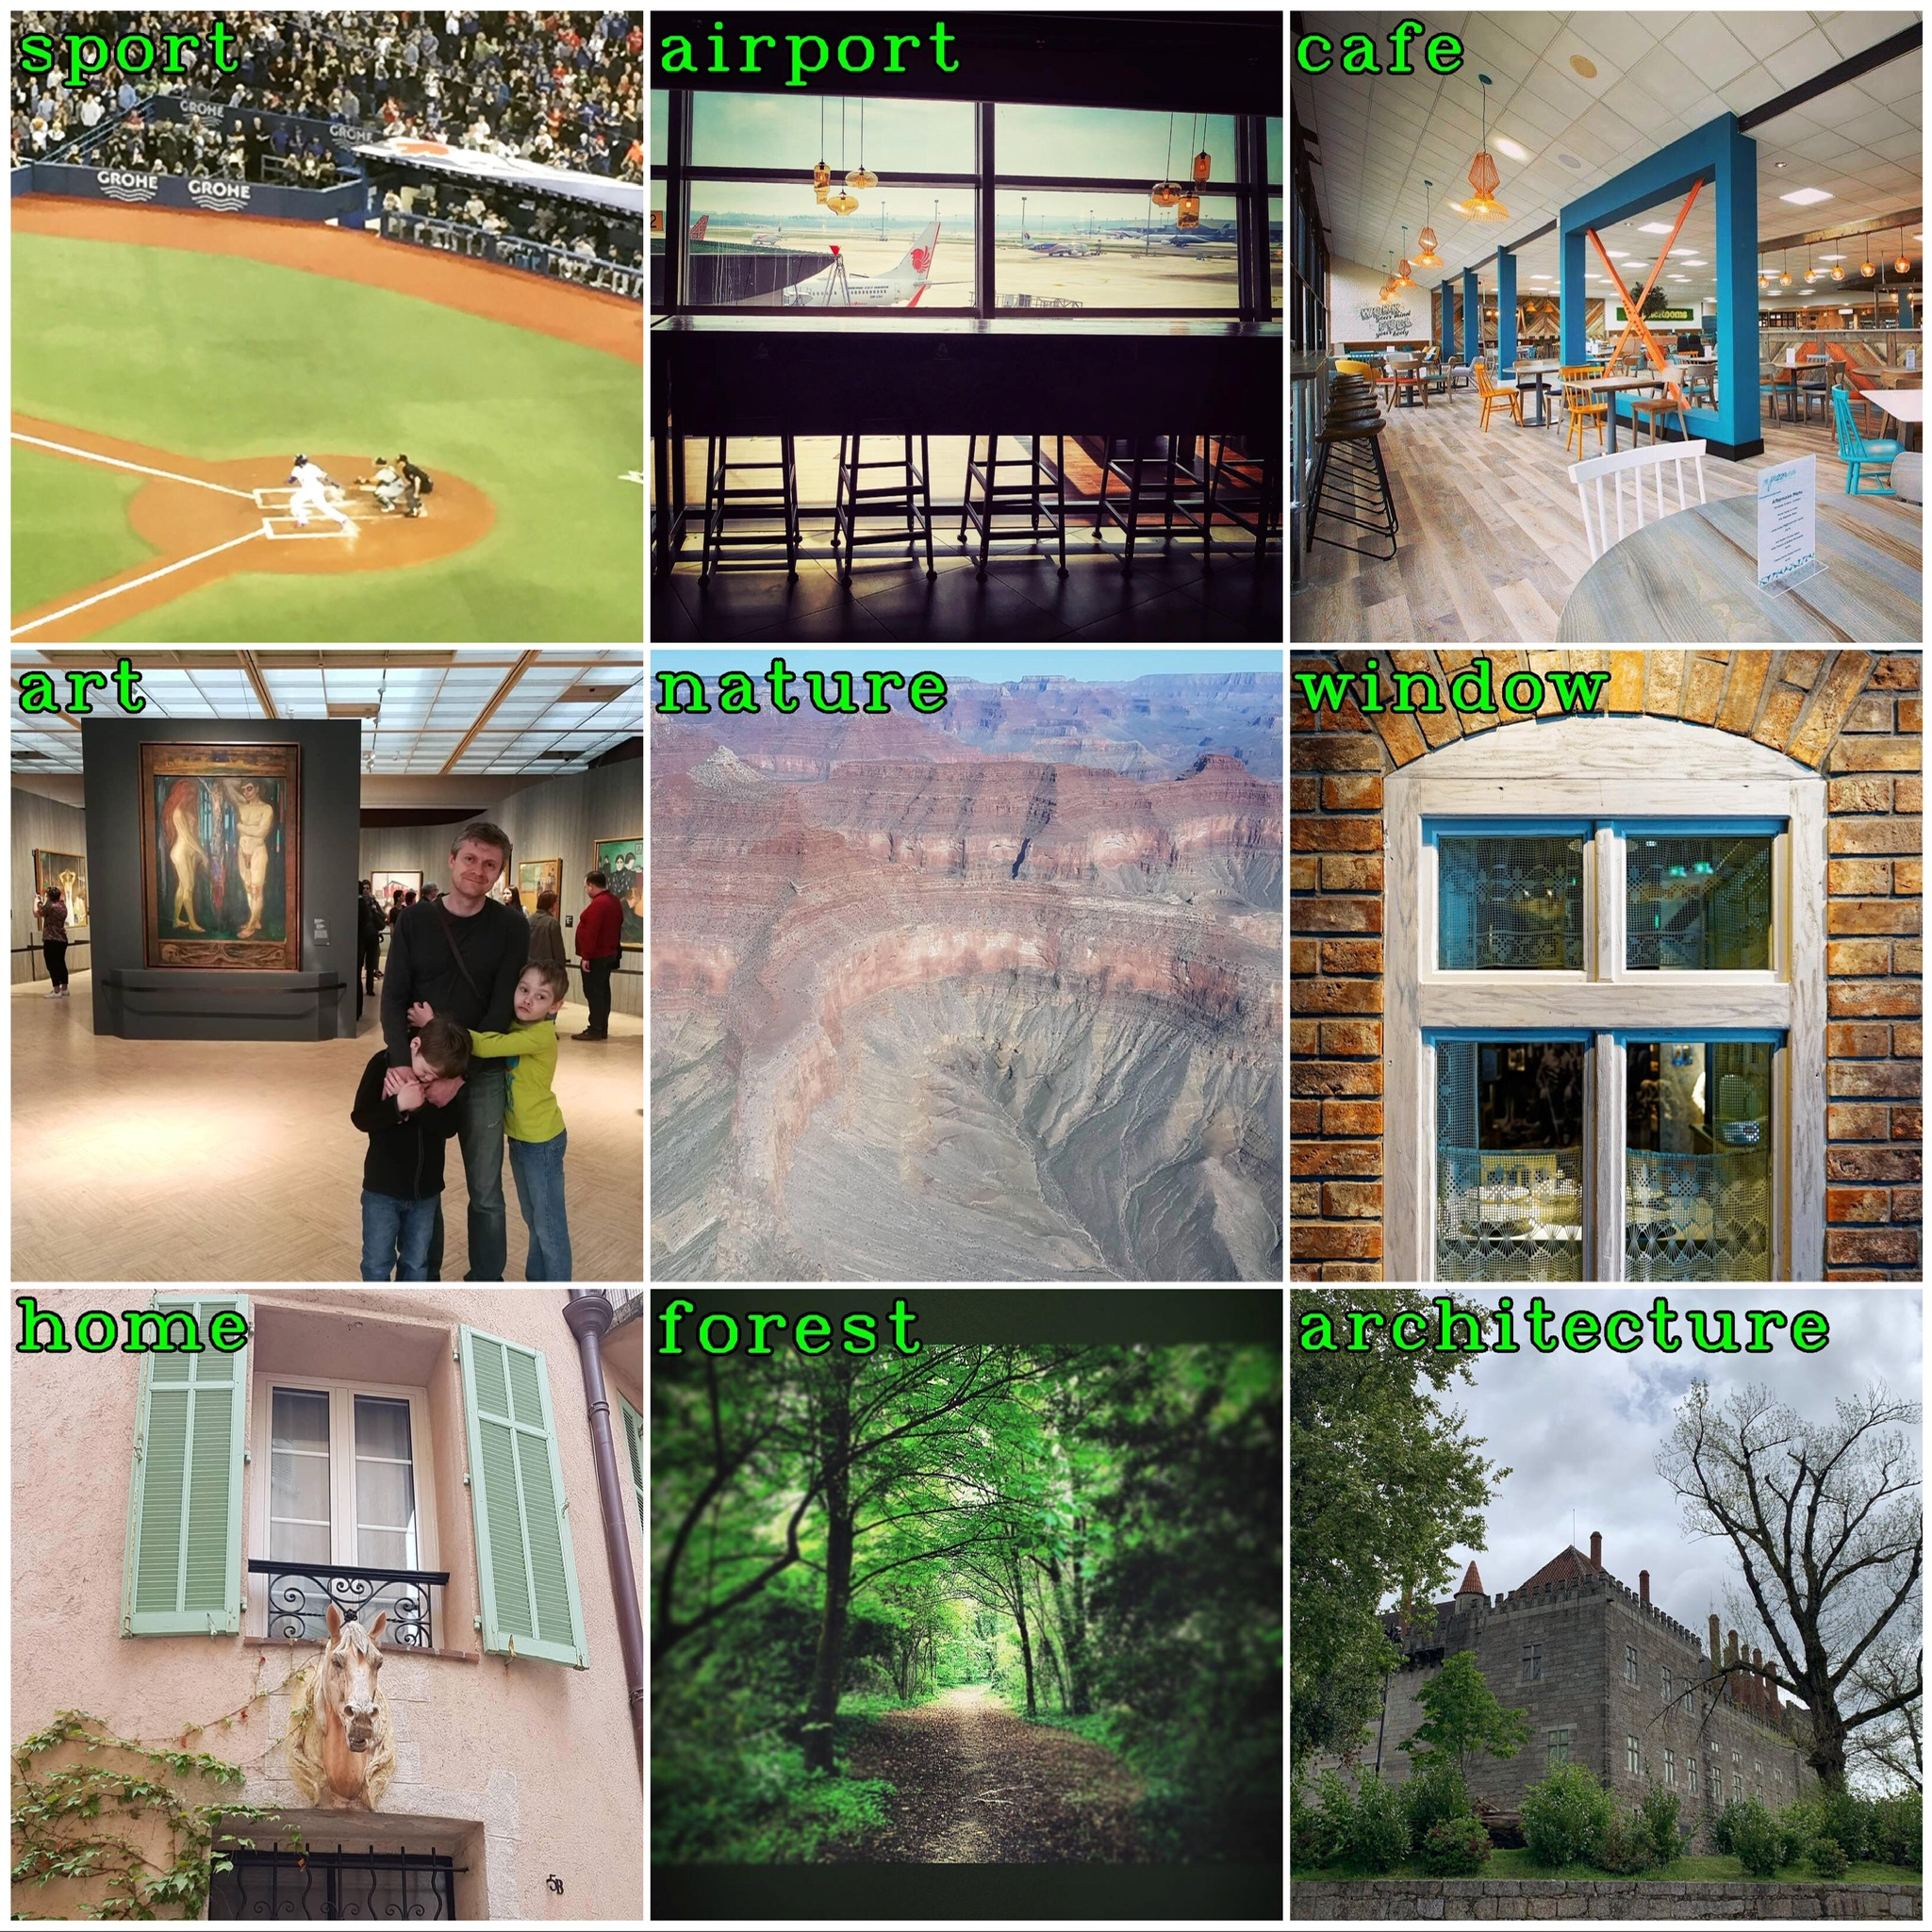
\includegraphics[width=0.75\linewidth]{insta_predict}
   	\end{center}
   	\caption{Примеры предсказаний для изображений из сети \textit{Instagram}.}
   	\label{tikzpicture: insta_predict}
\end{figure}


\indent
\indent
Далее для каждая пара изображение/предсказание была просмотрена человеком,
который принимал решение, подходит ли данное предсказание для изображения.
Значение точности модели (вычисленное в соответствии 
с выражением \ref{eq:accuracy}) оказалось равным 0.86; 
значение взвешенной точности (выражение \ref{eq:w_accuracy}) -- 0.83.


\indent
\indent
В завершении отметим, что произведенная процедура валидации может дать лишь
приблизительную оценку полезности построенной системы. Это объясняется
тем, что в процессе разметки может происходить некоторая подмена понятий.
Вместо действительно интересующего нас ответа о том, опубликует ли человек 
предложенный хэштег, мы можем получить ответ на другой вопрос --- 
соответствуют ли друг другу содержание изображения 
и предложенный хэштег. Ясно, что это разные вопросы, хотя и можно надеяться,
что ответы на них будут скореллированными.
К сожалению, получить точные оценки можно лишь внедрив 
предсказательную систему в продукт и собрав обратную связь.